\documentclass[11pt]{article}
\usepackage[a4paper, total={7in, 9in}]{geometry}
\usepackage[utf8]{inputenc}
\usepackage{amsmath, amssymb, stmaryrd}
\usepackage{hyperref}
\usepackage{caption, subcaption}
\usepackage{pdfpages}
\usepackage{float}
\usepackage{listings, color}
\usepackage{enumitem}
\usepackage{fancyhdr}
\usepackage[nottoc,numbib]{tocbibind}       % Including bibtex references in table of content
\usepackage{cleveref}
\usepackage[most]{tcolorbox}
\usepackage{varwidth}
\usepackage{multirow}
\usepackage{multicol}

% matthis.kruse@cispa.de

%%%%%%%%%%%%%%%%%%%%%%%%%%%%%%%%%%%
%    Commands for ease of use     %
%%%%%%%%%%%%%%%%%%%%%%%%%%%%%%%%%%%
\newcommand{\versionnr}{0.5}
\renewcommand{\*}{\cdot}                    % a pretty multiplication sign
\renewcommand{\implies}{\rightarrow}        % implies now is simple right arrow: -->
\newcommand{\lan}{\texttt{Japa} }
\newcommand*\lsin{\lstinline[columns=fixed]} % inline code blocks
\newcommand{\assigneq}{\oplus{\kern-5.0pt}=} % operator=

% Commands used during production
\newcommand{\rr}{(\textbf{\emph{REVIEW READY}})}
\newcommand{\dn}{(\textbf{\emph{DONE}})}
\newcommand{\ms}{(\textbf{\emph{MISSING}})}

%%%%%%%%%%%%%%%%%%%%%%%%%%%%%%%%%%%
%   Defining definition boxes     %
%%%%%%%%%%%%%%%%%%%%%%%%%%%%%%%%%%%
\newtcbtheorem[number within=section]{Definition}{}
{
        enhanced,
        sharp corners,
        attach boxed title to top left={
            xshift=-1mm,
            yshift=-5mm,
            yshifttext=-1mm
        },
        top=1.5em,
        colback=white,
        colframe=black,
        fonttitle=\bfseries,
        boxed title style={
            sharp corners,
            size=small,
            colback=black,
            colframe=black,
        } 
}{def}

\newenvironment{myDefinition}[2]{ \begin{Definition}[adjusted title=#1]{}{#2} 
    \textbf{Definition \thetcbcounter.} }{\end{Definition}}

%%%%%%%%%%%%%%%%%%%%%%%%%%%%%%%%%%%
%   Defining Theorem boxes        %
%%%%%%%%%%%%%%%%%%%%%%%%%%%%%%%%%%%
\newtheorem{theorem}{Theorem}[section]

%%%%%%%%%%%%%%%%%%%%%%%%%%%%%%%%%%%
% Defining a beautiful code block %
%%%%%%%%%%%%%%%%%%%%%%%%%%%%%%%%%%%
\definecolor{codegreen}{rgb}{0,0.6,0}
\definecolor{codegray}{rgb}{0.5,0.5,0.5}
\definecolor{codepurple}{rgb}{0.58,0,0.82}
\definecolor{backcolour}{rgb}{0.95,0.95,0.92}
\definecolor{bluekeywords}{rgb}{0.13,0.13,1}
\definecolor{greencomments}{rgb}{0,0.5,0}
\definecolor{redstrings}{rgb}{0.9,0,0}

\lstdefinestyle{mystyle}{
    backgroundcolor=\color{backcolour},
    commentstyle=\color{codegreen},
    keywordstyle=\color{magenta},
    numberstyle=\tiny\color{codegray},
    stringstyle=\color{codepurple},
    basicstyle=\ttfamily\footnotesize,
    breakatwhitespace=false,
    breaklines=true,
    captionpos=b,
    keepspaces=true,
    numbers=left,
    numbersep=5pt,
    showspaces=false,
    showstringspaces=false,
    showtabs=false,
    tabsize=2
}

\lstset{style=mystyle}

% CSS
\lstdefinelanguage{CSS}{
  keywords={color,background-image:,margin,padding,font,weight,display,position,top,left,right,bottom,list,style,border,size,white,space,min,width, transition:, transform:, transition-property, transition-duration, transition-timing-function},	
  sensitive=true,
  morecomment=[l]{//},
  morecomment=[s]{/*}{*/},
  morestring=[b]',
  morestring=[b]",
  alsoletter={:},
  alsodigit={-}
}

% JavaScript
\lstdefinelanguage{JavaScript}{
  morekeywords={typeof, new, true, false, catch, function, return, null, catch, switch, var, if, in, while, do, else, case, break},
  morecomment=[s]{/*}{*/},
  morecomment=[l]//,
  morestring=[b]",
  morestring=[b]'
}

%%%%%%%%%%%%%%%%%%%%%%%%%%%%%%%%%%%
%        Defining header          %
%%%%%%%%%%%%%%%%%%%%%%%%%%%%%%%%%%%
\pagestyle{fancy}
\lhead{\footnotesize Static Assertion Checking Optimization in a Janus-like
    programming language - version \versionnr}
\rhead{\today}


\begin{document}

%%%%%%%%%%%%%%%%%%%%%%%%%%%%%%%%%%%
%       Front page print          %
%%%%%%%%%%%%%%%%%%%%%%%%%%%%%%%%%%%
\includepdf[pages=1]{../../bachelor_project_description}
\newpage

\section*{Abstract}
A reversible programming language forces the programmer to write reversible programs, i.e.\
a program that can run in both direction; computing both from input to output, and output to
input. Reversible language are interesting to study, as it removes the theoretical lower limit
of heat generation, and that one only needs to write a single program, to handle functionality
that has a natural inverse, e.g.\ encryption. One downside to reversible language is, the added
overhead needed to guarantee correct behavior in both directions.

This thesis presents a optimizer module aimed at removing this runtime overhead. As the overhead
stem from runtime assertions, the presented optimizer tries to prove these assertions to always
hold using the satisfiability modulo  theory solver \texttt{z3}. To do this the thesis first
presents a simple imperative reversible language, similar to \texttt{Janus}. The optimizer
translates from this languages abstract syntax tree into a \texttt{z3} model, which is then
queried at every program point, that involves a runtime assertion. This thesis addresses some
of the complexion of this translation and querying to \texttt{z3}, when going from a reversible
language, e.g.\ the user defined possibly bogus runtime assertions.

This project shows that using the SMT solver \texttt{z3} to analyze reversible programs, in order
to remove the runtime overhead stemming from reversibility properties, is a doable. The SMT solver
utilizes the fact, that most assertions should always be true, unless the programmer wrote bogus
assertion, and is able to remove a significant amount of assertions. The biggest obstacle is
achieving the right amount of information to prove this validity.

This project showcase a complete translation from the \texttt{Janus} like language \lan to
\texttt{C++}, with a web interface for a broader field of application. This method could be useful
with further investigation into decreasing compile time, and utilizing statically known information
better, as these are the two main difficulties found during this project.
\newpage
\tableofcontents
\newpage

% Problem definition
% Boundaries
% What is reversable languages?
\section{Introduction}
Reversible programming languages allow the programmer to write programs, that can be run
both forward and backwards. Getting this ability into a language impacts the basic structure
such that assignments, conditional operations, and loops must be handled in another way
than traditional languages do. The reversibility of the programs does however have the benefits
of:

\begin{itemize}
    \item Lowering side-channel attack, as it does not constantly delete memory to make room for
    new information [FIND CITATION], thereby creating programs that generates a more constant
    stream of heat.

    \item Removing the theoretical lower limit of heat generation [FIND CITATION], making way
    for lowering the energy usage of computers (This does however require computers build
    for reversibility).

    \item Models the world of physics more precise, as physics in itself is reversible
    [FIND CITATION].

    \item Only needing to write one program, when functionality such as zip/unzip, that has
    a natural inversion that you want. This allows the programmer to write one program, prove
    correctness of one program, and then ship "two" programs.
\end{itemize}
\noindent
This project focuses on the last item for two reasons: 1) that the majority of computers today are
not reversible, and 2) that translating from a reversible language to an irreversible
generates certain overhead, as i.e. \texttt{if}-statements need both an entering condition and an
exiting assertion for reversibility; meaning the program needs to check an extra assertion each
time an \texttt{if}-statement is run.


\subsection{Boundaries}
The focus of this project is on finding whether a theorem prover is available for making static
program analyse in compile time, checking whether these extra assertions can be removed. Hence
there will be no other focus on optimization in the code generation
\\
\\
Also as this is a bachelor thesis the focus will be on freely available theorem provers.
% Definition of chosen language design and theory behind reversability
\section{Janus-like language definition}
This project alters and extents the syntax for \texttt{Janus} to make it better match modern
programming languages. This "new" language will be an imperative reversible language like
\texttt{Janus}, and henceforth will be noted as \texttt{JL} (short for Janus-like) in this report.
But before altering the syntax and functionality of \texttt{Janus}, a more formal characterizations
of reversibility must be made.
Reversible computation refers to the use of logically reversible transformations \cite{ARTICLE:2},
and require two things: Local reversibility and global reversibility.

\begin{myDefinition}{Local reversibility}{def:localReversibility}
For a local process to be reversible information from step to step must be preserved, meaning no
information is destroyed \cite{ARTICLE:1}.
\end{myDefinition}

\begin{myDefinition}{Global reversibility}{def:globalReversibility}
A global process can only be reversible if the mapping from a start state to a final state is
bijective \cite{ARTICLE:1}. 
\end{myDefinition}
\noindent
This means that every construct of \texttt{JL} must preserve information over time, so the program
knows where to start of when running in either direction, and that there must be a "one-to-one"
transformation from every state. e.g. consider the assignment operator \texttt{var = 10}. This
statement has no way of undoing itself, as we do not know what \texttt{var} was before this
assignment, meaning it goes against definition \ref{def:def:localReversibility}. It also removes
the bijective property of the program, as all previous states of \texttt{var} leads to the same
final state where \texttt{var == 10}.
\\
\\
The definition for logical reversibility stated above does allow for all programs to be reversible,
as one could simply save a copy of the initial state and final state, as this would make
the program bijective, as the final program becomes a tuple $(state_{initial}, state_{final})$,
making the program transformation $\{state_{initial}\} \to \{state_{initial}, state_{final}\}$.
These program will however not live up to Landauer's Principle, if every individual step is not
reversible. It is therefore imminent that all construct of \texttt{LR} are reversible in them self.

\subsection{Data types}

\subsection{Declaration of variables}
There are essentially two types of variables: Global and local. Because a global variable is
always in scope, it preserves the information at all time (assuming all operations done on it
are reversible). Hence global variable declaration can simply be done by:

\begin{table*}[h]
    \centering
    \begin{tabular}{lcl}
        \texttt{<id>} & $\underleftrightarrow{\text{Inverse of}}$ & no inverse \\
        \texttt{<id>[]}
    \end{tabular}
\end{table*}
\noindent
Local variables are mote tricky, as they will leave the scope, meaning we cannot know the value
of the variable when running the program backwards, if the variable have left scope. Hence there
needs to be some operation stating what the value of the variable is when it is last used, so
the program step of leaving the scope of a local variable also becomes reversible. This can be
done in the following way:

\begin{table*}[h]
    \centering
    \begin{tabular}{lcl}
        \texttt{<id>} & $\underleftrightarrow{\text{Inverse of}}$ & \texttt{delocal <id> == <expr}
    \end{tabular}
\end{table*}

\subsection{Modification arithmetics}
To modify a variable there needs to be a inverse function of the operator, such that the
modification can be reversed. As the only datatype for \texttt{JL} is integers, the only operators
with an inverse (the function is bijective) is addition, subtraction, and exclusive or.
Multiplication and division cannot be used, as they are not each others inverse when operating on
natural numbers. Hence the operation becomes:

\begin{table*}[h]
    \centering
    \begin{tabular}{lcl}
        \texttt{<id> += <expr1>} & $\underleftrightarrow{\text{Inverse of}}$ & \texttt{<id> -= <expr1} \\
        \texttt{<id> \textasciicircum= <expr2>} & & \texttt{<id> \textasciicircum= <expr2>}
    \end{tabular}
\end{table*}
\noindent
Where \textasciicircum ~indicates exclusive or.

\subsection{Arithmetics}
Performing arithmetics on expressions of the language does not require, that the arithmetic function
is bijective, as it is only the state transformations that need be bijective, e.g. in
\texttt{a += 5 $\*$ 6}, the expression \texttt{5 $\*$ 6} is not the "altering" function, and
inverse of the whole statement would simply be subtracting \texttt{5 $\*$ 6} from \texttt{a}.
\\
\\
The only thing one needs to remember is, that a variable name cannot occur at both side if the
statement is to be reversible. Having this constraint ensures forward and backward determinism
[FIND CITATION].

\subsection{Loops}
\texttt{JL} will support two different kind of loops: a \texttt{for}- and a \texttt{from}-loop.
The \texttt{from}-loop is identical to the one from \texttt{Janus}:
\newpage
\begin{table*}[!h]
    \centering
    \begin{tabular}{lcl}
        \texttt{from <expr1> \{} & $\underleftrightarrow{\text{Inverse of}}$ & \texttt{from <expr2> \{ }\\
        \texttt{ <stmts>} && \texttt{ <stmts>$^{-1}$} \\
        \texttt{\} until (<expr2>)} && \texttt{\} until (<expr1>)} 
    \end{tabular}
\end{table*}
\noindent
The \texttt{for}-loop is closer to \texttt{C++} syntax:

\begin{table*}[!h]
    \centering
    \begin{tabular}{lcl}
        \texttt{for <id> = <expr1> \{} & $\underleftrightarrow{\text{Inverse of}}$ & \texttt{for <id> = <expr2>; <inc>$^{-1}$ \{ }\\
        \texttt{ <stmts>} && \texttt{ <stmts>$^{-1}$} \\
        \texttt{\} <incr>; until (<id> == <expr2>)} && \texttt{\} until (<id> == <expr1>)} 
    \end{tabular}
\end{table*}
\noindent
Where \texttt{inc} is a modification operation typically on <id>, $a^{-1}$ indicated that
$a$ is reversed, and having \texttt{<inc>} above the body executes it before the body and
if it is after the body, it is executed after.
\\
\\
Moving the \texttt{<inc>} operation when reversing the loop is a necessity to make sure that
\texttt{<id>} always have to correct value when going into an iteration. If the operation was not
moved, the loop would be unaligned with its reversion. E.g. if the loop iterated over a list,
it might stop when \texttt{<id>} is equal to the length of the list. If we reversed without moving
the \texttt{<inc>} operation, the first iteration of the loop would access the index of the list
length, which would be out of bounds.

\subsection{If statements}
The \texttt{if}-statements are similar to those of \texttt{Janus}:

\begin{table*}[h!]
    \centering
    \begin{tabular}{lcl}
        \texttt{if (<expr1>) \{} & $\underleftrightarrow{\text{Inverse of}}$ & \texttt{if (<expr2>) \{} \\
        \texttt{ <stmts>} && \text{<stmts>$^{-1}$} \\
        \texttt{\} fi <expr2>} && \texttt{\} fi <expr1>} \\
        \texttt{else \{} && \texttt{else \{} \\
        \texttt{ <stmts>} && \text{ <stmts>$^{-1}$} \\
        \texttt{\}} && \texttt{\}}
    \end{tabular}
\end{table*}
\noindent
Where the \texttt{else} part can be omitted.

\subsection{Procedures}


% Getting constant into function calls

%

Now where all building blocks for procedures are reversible, it is straight forward to reverse
a procedure itself:

\section{Theorem Prover}
% Find representative set of theorem provers, and analyze in context of project
\subsection{Theorem Prover Versus Other Alternatives}
% Discussion over using theorem provers or partial evaluation?

\subsection{Choosing Theorem Prover}

\section{Compiler structure \rr}
The \lan compiler is structured into different modules that can be seen in figure
\ref{fig:compiler-overview}. First the \lan source code is handed as input to the frontend,
which creates an abstract syntax tree (AST), that is then type checked and annotated with
context sensitive information. This annotated AST is then reversed, giving us a reversed AST
$R(AST)$ and the regular. These two trees are then run through the optimizer, that outputs
two optimized trees, that is then translated into \texttt{C++} output via standard out.

\begin{figure}[h!]
    \centering
    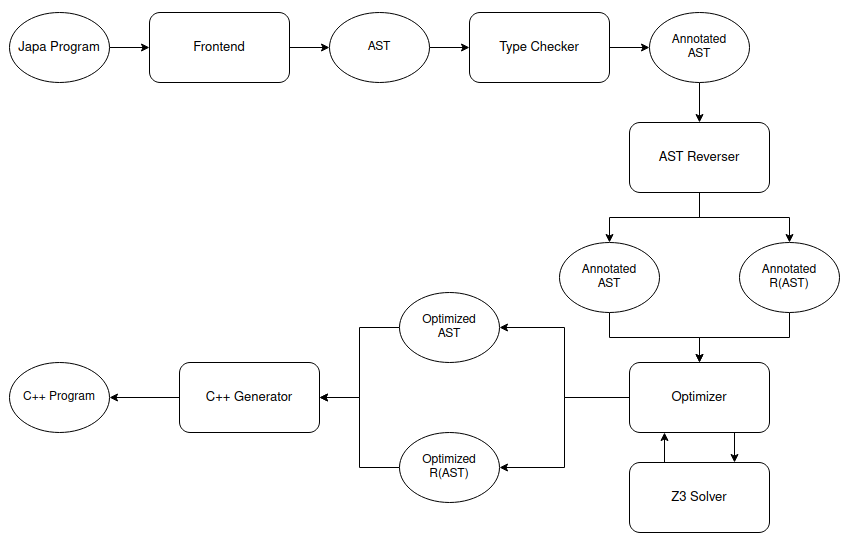
\includegraphics[scale=0.6]{imgs/compiler-overview.png}
    \caption{Compiler structure overview.}
    \label{fig:compiler-overview}
\end{figure}

\subsection{Frontend \rr}
% Theory and information behind lexing and parsing
The frontend consists of a lexical analysis and a syntax analysis. Both are implemented using a
parser combinator in \texttt{Haskell}, namely Parsec. A parser combinator is a higher-order
function taking in a parser as input, and outputting another parser. This way small simple parsers
can be combined into more complex structures, thereby helping quick prototyping. This strong
functionality does however come with a significant overhead, especially considering the simplicity
of \lan \cite{parser}.

The strong flexibility of parser combinators, and their strong resemblance of the underlying
grammar does however outweigh the negativity of the performance, especially considering this is
not the primary focus of this bachelor thesis.
\\
\\
Because the language is not in LL(1) the performance of the parser is also worsen, as lookahead
cannot be avoided e.g. in the distinction between simple variables and arrays, and the two
kinds of for-loops. The process presented in \cite{torben} can be used to transform it into
LL(1), but due to time constraints, this has been postponed to future works.
\\
\\
The parser combinator works on a string input on which it performs intertwined lexical analysis
and syntax analysis. The two analysis' are intertwined simply because that is how the Parsec
library functions. This does not pose any apparent problems, as the language being analyzed has
a fairly simple syntax. Parsec does however still keep a sense of modularity.

\subsection{Type checker \rr}
% Theory and information behind type checking
\lan is a statically typed language, as the type check is performed before execution of the program.
Furthermore, it is a strongly typed language, as operations are ensured to be performed on
types that are supported. The reason to make \lan a strongly typed language, as opposed to
the more weakly typed \texttt{C++}, which it is translated into, is that a strongly typed
language gives run-time guarantees that helps avoid certain type of program errors, that can be
hard to pinpoint during debugging, and even worse, might not even show up.
\\
\\
While type checking the AST two mappings are used to carry the type information synthesized by the
recursive calls onwards, so that the information can be inherited in other part of the AST; this
is a mapping from variable names to types, and from variable names to size. The latter is used
to annotate the AST with array sizes, that is needed during the subsequent optimizer phase.
No guessing of types are done during the analysis, meaning when an error is met it is reported
and the analysis stops.

\subsubsection{Type checking expressions}
When type checking expressions the symbol tables for variables and array size are inherited
attributes, and the type of expression, together with a annotated expression,
is the synthesized attributes. The rules for type checking
can be summarized as:

\begin{itemize}
    \item A number is simply an integer.

    \item A boolean value is a bool.

    \item The type of a variable is found by a lookup in the inherited variable table.
          If the lookup is successful the type is returned back, and if it fails a error
          is reported.

    \item The type of a lookup in an array is also determined by a lookup in the variable table.
          However, for array lookup the size needs to be annotated onto the expression, meaning
          a lookup into the array table is performed. If both are successful it is checked
          whether the array indexing is integers. If so the annotated
          expression is returned together with the type. Else an error is reported.

    \item For binary operations the type of the two expressions must match. As all types
          are defined for all operators, if the two types match the operator is checked in order
          to know what type it returns. If it is a boolean operator, the possibly annotated
          expression is returned together with the boolean type. Else the type of the expression
          is returned together with its annotated self. The choice that plus and multiply
          functions also for booleans is simply because \texttt{C++} does so.
        
    \item The type of the \lsin{not} expression is always boolean. Meaning the expression
          being inverted is simply checked, and then the possibly annotated expression is
          returned with the boolean type.

    \item The \lsin{size} expression always returns an integer, so the expression is simply
          returned with the integer type.
\end{itemize}

\subsubsection{Type checking statements}
Type checking statements involve the same inherited attributes, but here the synthesized are
the type/size annotated statement, and the updated tables.
The rules for type checking statements can be described as:

\begin{itemize}
    \item Variable definition and deallocation explicitly declare which type they are. Hence
          the check merely involves type checking the assigned expression, and see if it matches
          the declared type. If not an error is reported. Else the updated tables are returned
          together with annotated statement.

    \item For both simple types and arrays, the modification expression is checked if it matches
          the moderated variable. Array types the indexing expressions are also checked
          to be integers. If all is true, the updated tables are returned together with
          the now annotated statement. Else an error is reported.      

    \item A switch statement need to switch between two equal variables; so the types must match
          and if it is between arrays, the size of the arrays must also match. If these are not
          true, an error is reported, else the annotated statement together with the updated
          tables are returned.

    \item In conditional branching (if-then-else) both the if conditional, and the fi conditional
          must be a boolean type. Because these are statements and not expressions, the two
          branches do not have any "return" type, meaning the conditional rules are the only.
          So if they are true, the branch bodies are type checked, and the annotated statement
          is returned together with the inherited tables. Else an error is reported.

    \item In for loops the declaration, moderation, and deallocation needs to be type checked
          as explained above. Furthermore, the possible invariant needs to be a boolean type.
          If all that is true, the body is type checked, and an annotated statement is returned
          together with the inherited tables.

    \item Assertions simply needs to be a boolean type. If true the annotated statement is returned
          together with the inherited tables.
\end{itemize}


\subsubsection{Type checking procedure definitions}
Each procedure inherits the global store attributes, and uses this to type check its arguments,
and procedure body. Because there are no return types of procedures, it is only the arguments and
body, that needs type checking.

When all procedures have been type checked, the annotated AST is returned and used in the
subsequent phases of the compiler.

\subsection{AST reversing \rr}
The reverser simply follows the rules outlined under \nameref{sec:language-def}. The AST is
reversed at this point in the compiler, as the optimization checks needs to be performed for both
direction as explained in \ref{translation-to-z3}.

After the reversal each procedure should occur in the same order in the AST, but each
procedure body should be reversed. To achieve this the right associative \lsin{foldr} is used to
go through each procedure, and the left associative \lsin{foldl} is used within each procedure.
This can be seen in listing \ref{lst:reverser}. Notice that the first procedure in the AST is
skipped. This works under the contract, that the first procedure is always the \lsin{main}
procedure. The \lsin{main} procedure is not reversed because, it is used to define the start state
of the program. Hence it contains the global variables, which can only we 'reversed' if one were
to know the end state of the program, which would defeat some of the purpose of actually writing
the program in the first place.

\begin{lstlisting}[language=Haskell, label={lst:reverser}, caption={Reversing AST.}]
reverseProcedure (ProcDecl name args body pos) acc =
      let body' = foldl reverseStatement [] body in
            ProcDecl name args body' pos : acc

reverseProgram (Program ps) =
      let m = head ps in
            let rest = foldr reverseProcedure [] (tail ps) in
                  Program $ m:rest
\end{lstlisting}
\noindent
The methods for reversing statements are implemented as outlined in \nameref{sec:language-def},
but the implementeation for if-statements and for-loops will be descriped further here. These
can be seen in listing \ref{lst:stmt-reverser}. If-statements have their two conditionals switched,
such that the entrance conditional becomes the exit condition (from if path) and vice verser.
Then both paths are reversed recursively. With for-loops the expression of the loop variable at
entrance, is exchanged with the expression for the exit condition. Then the body is recursively
reversed.

Exchaning entrance and exit conditionals for the two constructs, guarantees that the reversed
statements bodies, will only be executed, if they were executed during the forward run. This
is illustrated in figure \ref{fig:rev-flow-constructs}; where reversal of the graph is done
by converting Diamonds to circles. circles to diamonds, squares to reversed squares, and at
last changing the arrows direction. Note that the reversible loop construct requires, that
the entrance condiotional be true, whenever the statement is executed. This is guaranteed in
\lan by using the for-loop construct instead of the from-loop, thereby making it possible to
exclude that runtime check.

\begin{lstlisting}[language=Haskell, label={lst:stmt-reverser}, caption={Reversing for-loops and if-statements.}]
reverseStatement acc = \case
      ...
      Ite condif bodyif condfi bodyelse pos ->
            Ite condfi
            (foldl reverseStatement [] bodyif)
            condif
            (foldl reverseStatement [] bodyelse)
            pos
            : acc

      For1 inv (Var t n (Just e) p) body mod cond b pos ->
            For2 inv (Var t n (Just cond) p) (reverseMod mod)
            (foldl reverseStatement [] body)
            e b pos
            : access
      For2 inv (Var t n (Just e) p) mod body cond b pos ->
            For1 inv (Var t n (Just cond) p)
            (foldl reverseStatement [] body)
            (reverseMod mod) e b pos
            : acc
      ...
\end{lstlisting}

\begin{figure}[H]
      \centering
      \begin{subfigure}[b]{0.4\textwidth}
            \centering
            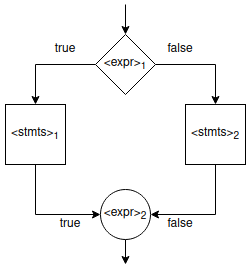
\includegraphics[scale=0.5]{imgs/reversible-conditional.png}
            \caption{Conditional.}
      \end{subfigure}
      \hfill
      \begin{subfigure}[b]{0.4\textwidth}
            \centering
            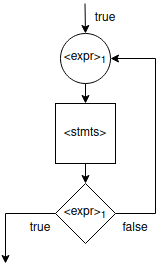
\includegraphics[scale=0.5]{imgs/reversible-loop.png}
            \caption{Loop.}
      \end{subfigure}
      \caption{Reversing conditionals and loop constructs.}
      \label{fig:rev-flow-constructs}
\end{figure}

\subsection{Optimization \rr}
% Strategy for optimization
% Integration with theorem prover
Because the compiler translates directly from the source language into an abstract syntax tree,
and then into \texttt{C++}, the optimization must be done on the abstract syntax tree, as it is
the easiest data structure to work on of the three. Doing the optimization directly on the source
language itself, saves the computation of translating to some intermediate language, but does
make this optimizer local to the source language.
\\
\\
This optimization involves four steps:
\begin{enumerate}
    \item Discovering language constructs, that require run-time assertions.
    \item Locating and gathering information for the prover.
    \item Translation of abstract syntax tree into \texttt{z3}.
    \item Deciding on whether to optimize the assertion or not, based on the answer
          from \texttt{z3}.
\end{enumerate}

\subsubsection{Language constructs requirering runtime assertions \rr}
The first point can be discovered by consulting the language specification introduced
in section \ref{sec:language-def}. Here it is imminent, that the following construct introduce
assertions for the translated code:
\begin{itemize} % TODO: Give example showing where assertions are created
    \item Deallocation of local variables.
    \item If statement as the program needs to know whether the if-path was chosen or not when
          reversing computations.

    \item For statement as the initial loop state must only be true at the initialization of the
          loop and never hereafter. This is the case, as it will function as the loop end
          condition, when reversing the statement.

    \item Assertions as it is in their nature.
\end{itemize}
\noindent
Which means that when running through the abstract syntax tree, the optimizer must stop and validate
when the above constructs are met, and then decide on whether to optimize based on the answer from
\texttt{z3}.

\subsubsection{Gathering information for \texttt{z3} \rr}
% Write more inticate details on loops e.g. how isdescending works, and how unroll works by using satisfy instead of validate
Point two has two main obstacles: 1) to know how much information \texttt{z3} needs for the proof,
and 2) granting the optimizer access to this appropriate subtree.

For 1) a simply approach could be to give the tree representing the current procedure to the
optimizer. This could give too much information in the sense that only part of this subtree is
actually needed to perform the validation check. e.g. in the small program, in listing
\ref{listing:z3-info-gather-ex}, the only thing
needed for the validation is the two last lines. However, this would require backtracking the
tree while keeping a list of "unassigned" variables, until this list is empty, so the first
method is used in this optimizer. For future work, it would be a good idea to check whether the
other approach would be faster. The below piece of code also reveal two other problem in regards
to information: Global variables and procedure calls.

To address this problem, the global store is processed before any optimization is performed.
In this way all procedures have access to this global store. \lan is statically scoped meaning
only the global store is available across procedures; this is the case as all procedures are
defined as the first thing in the program.
\\
\\
The information gathering is simply done locally for each procedure. Meaning when optimizing
a procedure \lsin{foo}, the only prior information is the global store. Then when a procedure
call for \lsin{bar} is met, \lsin{bar} is processed, so its information is carried out into
the analysis of \lsin{foo}. While doing this processing of \lsin{bar}, no optimization is done,
as that would use information from the call site, which could lead to spurious optimizations.
Because procedures are non-recursive this "inlining" can be done trivially without further
analysis.

\begin{lstlisting}[language=C++, label=listing:z3-info-gather-ex,
    caption=Example on gathering information for \texttt{z3} where only last two lines are needed.]
    int c

    procedure g()
    {
        c += 5
    }

    procedure f(int a)
    {
        call g()
        a += c
        local b = 1
        delocal b == 1
    }
\end{lstlisting}

\subsubsection{Handling if-then-else and for loop optimization \rr}
Conditional control-flow statements are the most complex to do a optimization run on, so they
will be explained further in the next two subsections.
\\
\\
\textbf{If-then-else}: As explained and outlined in section \ref{translation-to-z3}, the optimizer
cannot know statically which branch is going to be taken at run-time (at least for other than
trivial programs). Hence the translation must happen through the \texttt{z3} function
\lsin{mkIte}.

This function works by modelling each branch flow, and then "hiding" them both behind the
conditional decider. The code for this can bee seen in listing \ref{listing:ite}. What it does
is, that for each variable in the scope coming into the if-then-else, the variable is checked
in the two branches scope (the modeling of these scopes are processes prior to this) of whether
they have been "invalidated" by being removed (invalidation will be covered under loops below).
Then \lsin{mkIte} is used to base the decision on the variables value in the scope on the
if-conditional.

\begin{lstlisting}[language=Haskell, label=listing:ite, caption=Using \lsin{mkIte}.]
createITE :: AST -> Vars -> Vars -> Vars -> Z3 Vars
createITE cond orig scope1 scope2 = foldM f orig $ Map.keys orig
    where f scope name = do
            let var1 = tryGetVar name scope1
            let var2 = tryGetVar name scope2

            case (var1, var2) of
            (Just (var1z3, var), Just (var2z3, _)) -> do
                newVar <- makeVar (fromJust (getVarType var)) name
                ite    <- Z3.mkIte cond var1z3 var2z3
                Z3.assert =<< Z3.mkEq newVar ite
                return $ Map.insert name (newVar, var) scope

            -- else variable invalidated in some scope
            _ -> return $ Map.delete name scope
\end{lstlisting}
\noindent
\textbf{Loops}: \texttt{Z3} does not have a theory for handling loops. A loop must therefore be
reformulated for \texttt{z3}, as mentioned in section \ref{translation-to-z3}. The optimizer
has three different cases in which some information can be transferred to \texttt{z3}: 1)
Loop has invariant attached and can be unrolled, 2) loop cannot be unrolled but has invariant,
and 3) loop does not have an invariant attached but can be unrolled. For all other combinations
it is, to the best of my knowledge, not safe to carry information to \texttt{z3}, as we cannot
paint the whole picture. An example for this is, if it is conveyed that $x = c_1$ to \texttt{z3}
prior to the loop, and the loop would ensure $x=c_2$, but we have no way of statically getting this.
If the information of $x=c_1$ was then carried on past the loop, it could result in faulty
optimizations. Invalidating $x$ is done by replacing the \texttt{z3} var representing the value
of $x$, by a new \texttt{z3} variable, of which we know no more than it's existence; this way
no prior information, which now may be invalid, is carried onwards in the analysis.

Determining whether loops are unrollable is done with the simple method, of 
\begin{enumerate}
    \item Checking that the initial value, the loop modifier, and the deallocation are based on
          simple constants.

    \item No modification of the loop variable should be performed during the loop body execution.

    \item The loop should not be based on integer overflow/underflow.

    \item The loop unroll number does not exceed an arbitrary given bound (simply to not let
          the recursively loop "forever").
\end{enumerate}
\noindent
If all above criterions are met, the loop is deemed unrollable, and the loop will be unrolled.
Otherwise all modified variables within the loop are invalidated, except for those in
the loop invariant.

In order for an invariant to help carry information past a loop that cannot be unrolled, it needs
to be true at initialization of the loop, during maintenance, and the loop should terminate.
The three criterions are validated by:
\begin{itemize}
    \item \emph{Initialization} is simply proved by validating the invariant before the loop starts.

    \item \emph{Maintenance} is proved by processing a run of the body and modification, on a
          generalized scope, and then validating the invariant. If the invariant is true for this
          general case, it will be true for all iterations. The generalization of the scope is
          done by "invalidating" the entire scope.

    \item \emph{Termination} is proved by validating that after a general run of the loop,
          the loop variable will be either strictly larger or smaller than before, depending
          on the loop modifier.
\end{itemize}
\noindent
Loop unrolling is only done to enable exact information for the \texttt{z3} solver. It has nothing
per se to do we the speed of the resulting code (ignoring the fact that missing information
might lead to assertions not being removed). Therefore, if the optimizer is given a nested loop,
if the inner loop cannot be unrolled, there is no use in unrolling the outer loop. Information will
be invalidated no matter what. Furthermore, as a matter of running time for the optimizer, there
is an arbitrary bound of the amount of unrolling done. Meaning if a loop requires 31 unrolls, but
the max is 30, the loop is not unrolled. Hence the inner loop is unrolled first, and then the outer
loop. If the inner loop requires 10 unroll, and the outer can be unrolled 5 times, the total
required unrolling of the outer is $10*5$. To further lessen the burden on the \texttt{z3}
solver, the function \lsin{satisfiable} is used instead of \lsin{validate} for the loop
variable assertions. This is the case, as the semantics of \lan forces this generated assertion
to be non bogus, meaning it is not needed to do the additional check of whether the expression
is bogus.
\\
\\
If a loop is deemed to not be unrollable, a generalized analysis of the loop will be performed.
This means the loop optimizer will be run on a generalized scope. The code snippet
\ref{require-generalize} shows an example, where this generalization is necessary to get the
correct result. If it was run once in the normal scope, the if path would not be considered,
meaning the for-loop would be optimized. But if \lsin{tmp} and \lsin{i} is generalized, the
optimizer will correctly state, that the loop is not optimize-able.
Generalizing the scope is done for all variables, that are modified within the loop body;
this also includes the loop variable.

\begin{lstlisting}[language=C++, label=require-generalize, caption=Loop requirering generalization]
int tmp = 0
for local int i = 0 {
      if (i == 3 && tmp == 0) {
            i -= 3
            tmp += 1
      } fi (i == 0 && tmp == 1)
} i += 1, until (dealloc int i = 4)
\end{lstlisting}
\noindent
This loop optimization based on a generalized scope can be seen in listing
\ref{lst:generalizeLoopOpt}.
First every variable that will be modified within the loop body is generalized, for the
reasons explained above. Then the compiler tries to validate whether the loop variable is
increasing or decreasing. This is used in order to put in more information about to loop
variable for the generalized run. If this step was omitted, many optimization could not be
done, as the generalized loop cannot guarantee that the loop variable does not overflow/underflow.
Hence guaranteeing that the loop variable will never reach the initial value again at the end
of an iteration becomes almost impossible; without the information from the
\lsin{loopDescending} call.
Then the statement body is optimized (if we are running optimization round), 
by calling \lsin{unroll} with \lsin{doOpt}. This then reveals whether the assertion
created by the loop variable, can be optimized away in a generalized environment.

\begin{lstlisting}[language=Haskell, label={lst:generalizeLoopOpt},
      caption={Optimizing the loop based on generalized information.}]
generalizedAnalysis scope body z3expr m state warnings = do
      -- Generalize all variables in scope, and check for validity
      tmpScope <- invalidateVars scope $ modifiedVars ast body

      -- Trying to get more information about the loop variable
      let loopVar = fst $ fromJust $ tryGetVar name tmpScope
      loopDirection <-
            loopDescending scope forward var m body state bound warnings
      (case loopDirection of
            Ascending  -> Z3.assert =<< Z3.mkBvuge loopVar z3expr
            Descending -> Z3.assert =<< Z3.mkBvule loopVar z3expr
            Unknown    -> return ())

      (body', _, validated, warnings') <-
            unroll 1 doOpt forward body pos var z3expr m tmpScope state warnings
      return (tmpScope, body', validated, warnings')
\end{lstlisting}

\subsection{Translation to \texttt{C++} \rr}
The \lan compiler presented in this report does a simple translation to \texttt{C++}.
As the focus lie on assertion removal, no work has been put into compiling effective
\texttt{C++} code. The main function of the code generator can be seen in listing
\ref{lst:formatMain}. It works by receiving two AST's: One forward direction and one reversed.
It starts by inserting includes possibly required by the translated code. This includes

\begin{itemize}
      \item \lsin{assert.h} to enable use of asserts in the \texttt{C++} code.

      \item \lsin{cstring} to get access to \lsin{memcmp} functionality, which is used
            when deallocating array variables.
\end{itemize}
\noindent
Then it formats the starting global store of the \lan program. This is put into the global
scope, so that they can be accessed freely from all functions. Because the main procedure of
the \lan program, is not reversed, it simply takes the one obtained from the forward AST
(here the first parameter).

Then function definition is created for all procedures of the program. This is done as
functions in \texttt{C++} can only be called after their declaration, whereas in \lan
they can be called, as long as they are in the global scope.
After this all procedures are formatted into \texttt{C++}.

\begin{lstlisting}[language=Haskell, label={lst:formatMain}, caption={Formatting AST into \texttt{C++}}]
formatProgram :: Program -> Program -> Doc
formatProgram (Program ps) (Program psR) =
      case zip ps psR of
      (main:tl) ->
      formatIncludes
      $+$ space $+$
      formatGlobalVars (getProcDeclBody (fst main))
      $+$ space $+$
      foldr formatProcedureDefinition empty tl
      $+$ space $+$
      foldr formatProcedure' empty tl
      $+$
      formatProcedure (fst main)
      [] -> empty
\end{lstlisting}
\noindent
Formatting procedure declarations are straight forward, as every procedure must return void.
The only thing is, that parameters are all passed by reference instead of values; for
normal variables this allows to alter the value within it; for arrays is avoids decaying the
variable to a pointer to first element. Decaying to a pointer is avoided, so the function
\lsin{sizeof} can still be used, even on array parameters. If the array was passed as value,
it would be decayed to \lsin{int*} meaning \lsin{sizeof} would return $8$ (depending on the
architecture).
\\
\\
When transforming the different statement constructs into \texttt{C++}, the following rules
are implemented:
\\
\\
\textbf{Local variables declaration, modification, and deallocation:}
Local variable declaration and modification are simply translated into regular variables and
assignment modifications in \texttt{C++}, as they behave
similarly. The only difference is, that \lan local variables needs to be deallocated at some
point. This deallocation is translated into \texttt{C++} assertions, as they behave as a
program runtime check.

deallocation of arrays are somewhat more complicated, as arrays in \texttt{C++} cannot be
declared inline in an assert. Hence a temporary array $_tmp_arr$ is created, with the values
stated in the deallocation statement, and is compared to the values of $arr$, by using
\lsin{memcmp}; as \lsin{memcmp} has no check for array length, this is checked before the
call, using the short-circuiting operator $\&\&$.
\\
\\
\textbf{Switch:}
At the moment switch statements are translated into a series of exclusive-or bitwise operations.
This is faster than creating a temporary variable to hold, the value of one of the variables, 
while during the switch. However, it does alter the behavior if the two variables being
switched aliases each other. Here the exclusive-or operations will simply zero-initialize
the two variables, instead of switching the values. This should be altered in the future,
unless guarantees can be made that the variables are non-aliasing.
\\
\\
\textbf{If-then-else:}
The only semantic difference between \lan conditional statements and \texttt{C++} ones,
is the runtime assertion from the \lsin{fi}, that should be true whenever the \lsin{if}
branch has been run. Hence the translation simply involves, transforming to a simple
\texttt{C++} if statement, with accompanying assertion of the \lsin{fi} expression, in the
if-branch.
\\
\\
\textbf{For loops:}
\lan for-loops are transformed into a while-loop. While-loops are chosen instead of for-loops
as \lan for-loops can alter whether the loop variable should be modified at the start of an
iteration or at the end. During the translation assertions can occur at the following
destinations:
\begin{enumerate}
      \item \label{en:init} After loop variable initialization, if there is an invariant and it isn't proven.
      \item \label{en:main} At the start loop body, if an invariant is given and not proven.
      \item \label{en:body} At the end of the loop body if loop could not be proven
      \item \label{en:term} After the loop construct, if invariant is present and not proven.
\end{enumerate}
\noindent
In order to keep track of which assertions should be formatted, and which have been proven
away, the data construct \lsin{data LoopInfo = LoopInfo Bool Int}. The bool indicates whether
assertion \ref{en:body} above should be present or not. All invariant based assertions are
tracked via the \lsin{LoopInfo} integer; the least significant bit indicated whether
assertion \ref{en:init} should be formatted; the next whether assert \ref{en:main} should
be formatted; the next whether assertion \ref{en:term} should be present. If the bit is
$1$ the invariant assertion should be formatted, else it has been proven always valid.
\section{Testing of compiler \rr} \label{sec:tests}
%Also add the example of failing test
Testing of the compiler is done in two ways: Automatic and manually. Automatic tests is
done by running the compiler, inspecting the output code, running the output using \texttt{g++},
manually writing the prober model in \texttt{z3}, and then if it all works, a gold file is
created with the output code, and the test then checks the output of the compiler against this
gold file. This method is used, to track any regression in the code output. This is done, as
the main function of the compiler is to optimize the code.

Manual tests were conducted during production of the different modules. This simply involved
running the code in \texttt{ghci}, and printing out each step of the way; prototyping towards
the end compiler.
\\
\\
The automatic tests are run using the bash script from listing \ref{lst:tester}. The test
script goes through every test \lan file, and compares the output with the corresponding
gold file. \lsin{2>&1} is used to direct both standard in and standard out from the compiler
run, so that negative tests, can also be created. If the two files match a green text
is written with "Success".

There are $32$ test programs that cover a small set of edge cases. Currently all test programs
are successful except for one. An image of a test-run can be seen in figure \ref{fig:testrun}.
The failing test is \texttt{factorial-overflow.japa}, and it fails as the compiler wrongfully
removes an assertion that should not be removed. The optimizer wrongfully says that the assertion
created by the \lsin{dealloc} in the forward direction can be removed. There was not enough time
to find the root cause of this issue, so it is left for future work.


% Talk about how testing could have been improved
\begin{lstlisting}[language=Bash, label={lst:tester}]
...
compare () {
    if [ -f $2 ]; then
        local expected="$(cat $2)"
        if [[ "$output" != "$expected" ]]; then
          echo "Output for $0 does not match gold file."
          echo "Compare $1 with $2."
          return 1
        else
            return 0
        fi
    fi
    echo "gold file ($2) not present"
    return 1
}

...

for f in $test_dir/*; do
    fname="$(basename "$f")"
    program_name="$(echo $fname | sed 's/.japa$//')"
    printf "%*s" $file_len " $fname:  "

    # Save both stderr and stdout in output, so negative tests can also be tested
    output=$($compiler $f 2>&1)
    if compare $fname "$gold_dir/$program_name.gold"; then
       echo -e "\033[92mSucess.\033[0m"
    else
       echo -e "\033[91mTest error.\033[0m"
    fi
done
\end{lstlisting}
\section{Benchmark of compiled code \rr}
To asses the impact of the optimization run done by the \lan compiler, the
example programs presented in the we interface, except for the "unrollableLoop" program.
However, extra loops calling and uncalling each function are inserted to make the programs
more demanding, creating hot loops
(see \ref{sec:benchmark-programs}). Two factors are used to asses the impact: 1) compile time
of program, and 2) running time of compiled program. For the latter the output \texttt{C++}
program is translated to machine code using the \texttt{g++} compiler, version $9.4.0$
for \texttt{Ubuntu}. No extra optimizations is done using the \texttt{g++} compiler, to
isolate the pure impact of the \lan compiler optimization.
\\
\\
To benchmark compile time the \texttt{Criterion} \texttt{Haskell} package has been used,
and the benchmark is build using \texttt{Cabal}. Because the \lan compiler utilizes
standard out and standard error, to output its result, a small command is written in the
\texttt{Makefile} to suppress information that is not needed for the benchmark. Hence
to benchmark the compile time with and without optimizations, use the given
\texttt{Makefile} using the command:
$$\texttt{make bench}$$
\noindent
Benchmarking the runtime of the output program is done using the supplied \texttt{bash}
script \texttt{runbenchmark.sh} (see appendix \ref{lst:runbenchmark}). This simply compiles
the \lan compiler to ensure newest edition, compiles executable for each benchmark program,
and then executes each 10 times and reports the average.
\\
\\
The results of the benchmark can be seen in table \ref{table:benchmark-results}.
It should be noted that binary size is calculated using lines of assembly, and not the
actual size in KB of the binary file. This is done, as number of assembly lines is a
more direct measure of the \lan compiler optimizations. The difference is calculated as
the percentage increase from no optimization to optimizations.

\begin{table}[H]
    \centering
    \begin{tabular}{|l||r|r|r||r|r|r||r|r|r|}
        \hline
        \multirow{2}{*}{Program}& \multicolumn{2}{c|}{Compile Time (ms)} & \multirow{2}{*}{Diff (\%)} & \multicolumn{2}{c|}{Runtime (ms)} & \multirow{2}{*}{Diff (\%)} & \multicolumn{2}{c|}{Binary Size} & \multirow{2}{*}{Diff (\%)} \\
        \cline{2-3} \cline{5-6} \cline{8-9}
        & \multicolumn{1}{c|}{(noOpt)} & \multicolumn{1}{c|}{(opt)} & & \multicolumn{1}{c|}{(noOpt)} & \multicolumn{1}{c|}{(opt)} & & \multicolumn{1}{c|}{(noOpt)} & \multicolumn{1}{c|}{(opt)} &  \\
        \hline
        Fibonacci    & $0.6526$ & $5741.00$ & $879611.92$ & $4.79376$ & $4.080000$ & $-14.89$ & $249$ & $171$ & $-31.33$ \\
        \hline
        Factorial    & $0.3725$ & $119.70$  & $32034.23$  & $2.08916$ & $1.81717$  & $-13.02$   & $211$ & $160$ & $-24.17$ \\
        \hline
        Perm to code & $0.6481$ & $70.25$   & $10739.38$  & $1.81760$ & $1.74201$  & $-4.16$  & $264$ & $192$ & $-27.27$ \\
        \hline
    \end{tabular}
    \caption{Results from benchmark. Diff is calculated as percentage increase from no optimizations
    to optimizations enabled.}
    \label{table:benchmark-results}
\end{table}
\noindent
So on average, for the three programs, the \lan compiler is able decrease the amount of
assembly lines by $27.76\%$. Which also shows in the fact, that all programs run faster with
optimization on, than without. Listing \ref{lst:benchmark1} shows the \texttt{C++} code of
running with optimizations and none. This shows that the optimizer was able to remove all
assertions inserted by the reversibility of \lan for the Fibonacci program. The fact that
the runtime of the Fibonacci program benefits the most from the optimizations, stems simply
from its deeper loop structures. Meaning more amount of iterations, the more important are
the optimizations.
\\
\\
The compile time for all three programs, are increased significantly by performing optimizations.
On average the compile time increases with $354367.49\%$, which does lengthen iteration time
when developing software. Furthermore, all three programs are short and relatively simple,
meaning for more complex programs, the compile time difference might increase further.
Therefore, it is not advisable to use optimization during development, but wait for the
release build.
\\
\\
Further work should include focus on developer iteration time instead of code generations,
to test the viability of these optimizations in a developer environment. Profiling the execution
of the compilation shows, that most time is spend in the optimizer, meaning a focus could be
on focusing the optimization for hot code segments, thereby keeping most runtime gains while
hopefully decreasing execution time. Actually, for the Fibonacci program, approximately
$32\%$ of the time is spend on optimizing forward directional part of the program, and
approximately $69\%$ is used on optimizing the backward directional part of the program.
This happens even though the reverse actually skips optimizations for the \lsin{main}
procedure. Hence if the reason for this increase could be found, a good chunk of the
execution might be removable. The fact that the reversed fib is significantly slower
to optimized than the non-reversed, might hint that the \texttt{z3} solver has a harder
time picking the appropriate solvers, based on the information it is given, so it might
end up picking a solver, that directs it in a less efficient direction of the solver-tree.

\begin{varwidth}[t]{0.45\textwidth}
\begin{lstlisting}[language=C++, caption={Optimized Fibonacci program.}]
...
// Global variables defining starting state
unsigned int x1 = 0;
unsigned int x2 = 1;
 
...

void fib_forward(unsigned int &x1, unsigned int &x2, const unsigned int n)
{
    unsigned int i = 1;
    while(i != n)
    {
        unsigned int tmp = (x2) - (x1);
        x2 += x1;
        x1 += tmp;
        i += 1;
    }
}
 
void fib_reverse(unsigned int &x1, unsigned int &x2, const unsigned int n)
{
    unsigned int i = n;
    while(i != 1)
    {
        i -= 1;
        unsigned int tmp = (x1) - ((x2) - (x1));
        x1 -= tmp;
        x2 -= x1;
    }
}
 
int main()
{
    unsigned int i = 0;
    while(i != 1000)
    {
        fib_forward(x1, x2, 200);
        fib_reverse(x1, x2, 200);
        i += 1;
    }
}
\end{lstlisting}
\end{varwidth}
\hspace{4em}
\begin{varwidth}[t]{0.45\textwidth}
\begin{lstlisting}[language=C++, caption={Unoptimized Fibonacci program.}]
... 
// Global variables defining starting state
unsigned int x1 = 0;
unsigned int x2 = 1;
 
...
 
void fib_forward(unsigned int &x1, unsigned int &x2, const unsigned int n)
{
    unsigned int i = 1;
    while(i != n)
    {
        unsigned int tmp = (x2) - (x1);
        x2 += x1;
        x1 += tmp;
        assert(tmp == (x1) - ((x2) - (x1)));
        i += 1;
        assert(!(i == 1));
    }
}
 
void fib_reverse(unsigned int &x1, unsigned int &x2, const unsigned int n)
{
    unsigned int i = n;
    while(i != 1)
    {
        i -= 1;
        unsigned int tmp = (x1) - ((x2) - (x1));
        x1 -= tmp;
        x2 -= x1;
        assert(tmp == (x2) - (x1));
        assert(!(i == n));
    }
}
 
int main()
{
    unsigned int i = 0;
    while(i != 1000)
    {
        fib_forward(x1, x2, 200);
        fib_reverse(x1, x2, 200);
        i += 1;
        assert(!(i == 0));
    }
}
\end{lstlisting}
\end{varwidth}
\section{Packing compiler }
The \lan compiler is written in \texttt{Haskell} using the \texttt{cabal} packaging system
\cite{cabal}. Therefore, the \texttt{.cabal} file located in the root of the package, indicate
the structure of the program. The structure of the program can be seen in
\autoref{fig:structure}. It consists of $3352$ lines of \texttt{Haskell} code, $197$ lines of
bash code, and some \texttt{html}, \texttt{PHP}, \texttt{css}, and \texttt{javascript}.

\begin{figure}[H]
    \centering
    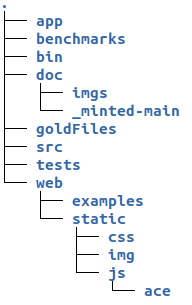
\includegraphics[scale=0.7]{imgs/directory-structure.png}
    \caption{Directory hierarchy of \lan package, printed out using \lsin{tree}.}
    \label{fig:structure}
\end{figure}
\noindent
The directory hierarchy holds the following purpose:

\begin{itemize}
    \item The \texttt{src/} folder contains the \lan library code, and \texttt{app/} contains a
          simple executable of the compiler. This division is used, in order to allow other
          packages to import and use different parts of the \lan compiler.

    \item \texttt{benchmarks/} contains the benchmark
          programs, the \texttt{cabal} benchmark file \texttt{HaskellBenchmark.hs}, and the
          \texttt{bash} script handling the execution time benchmarks.
    
    \item \texttt{bin/} contains the \lan executable and the \texttt{bash} test script.

    \item \texttt{doc/} contains the \LaTeX ~source files for this report.

    \item \texttt{goldFiles/} contains all the gold files used during testing, and
          \texttt{tests/} contains all the \lan test files.

    \item \texttt{web/} contains the source code for the \lan playground webpage. Within this
          directory \texttt{examples/} contains the example programs used in the playground,
          \texttt{static/} holds all the \texttt{javascript}, \texttt{css}, and images
          used for the interface. \texttt{web/} itself holds the \texttt{PHP} scripts
          handling the communication between the web page and the underlying server;
          meaning calling the \lan compiler and loading example programs.
\end{itemize}

\subsection{Compiler package and usage }
% Installation, requirements, usage
As before mentioned the \lan package is created using \texttt{cabal}. Hence it can be constructed
using the regular \texttt{cabal} commands.
In order to build the compiler, \texttt{cabal} version $2.4$ is required. To install the
required dependencies issue the \texttt{cabal install} command.
A \texttt{Makefile} is included within
the root directory, that contains commands for 1) building the compiler, 2) testing the compiler
3) benchmarking the compiler. To perform these functions simply issue the commands below from
the root directory:
\begin{enumerate}
    \item \texttt{make}
    \item \texttt{make test}
    \item \texttt{make bench} or \texttt{make benchR}
\end{enumerate}
\noindent
All of the above will build the compiler anew, and create an executable \texttt{japa} in the
\texttt{bin/} directory.
\\
\\
The web-based \lan playground can be run using \texttt{PHP}. To boot up a local web server,
navigate to the \texttt{web/} directory and run:
$$\texttt{php -S localhost:<port number>}$$
\noindent
This will start a process running the web server on your localhost IP, on port $<port number>$.
Now simply navigate to a browser, and paste \texttt{localhost:<port number>} into the search bar,
and you will be taken to the webpage.

\subsection{Web interface for compiler }
The web interface is based upon that of the \texttt{Janus} playground \cite{janusInterp} from
the bachelor thesis written by Claus Skou Nielsen and Michael Budde \cite{janusPlayground}.
The code has merely been altered to fit the purpose of the \lan showcase. Hence the only
modifications are within:

\begin{itemize}
    \item \texttt{index.html} to split the window vertically instead of horizontally,
          because the purpose of the webpage is to showcase the output \texttt{C++}
          code, and not interactively write \lan code. Some buttons has also been
          removed or altered.

    \item \texttt{execute.php} to not run an interpreter, but to run the \lan compiler
          on the input program in the playground.

    \item \texttt{playground.js} to follow the new format and functionality of the playground.

    \item \texttt{playground.css} to make the \texttt{css} match the new functionality with
          the vertical split.

    \item \texttt{mode-janus.js} to make syntax highlighting match \lan and not
          \texttt{Janus} syntax.
\end{itemize}
\noindent
It is indicated in each file, what has been created for this project, by outlining them
in comments such as:
\begin{lstlisting}
///////////////////////////////   "new"  //////////////////////////
some code
////////////////////////////// "new" end //////////////////////////
\end{lstlisting}
\noindent
An image of the \lan playground can be seen in \autoref{fig:japa-playground}.
The left pane view is a textarea that takes in the \lan program. The right pane view
displays the compiled \texttt{C++} code. To compile a \lan program simply insert the program
in the left view, press the green button that says \texttt{C++}, and wait for it to show
in the right pane. A small number of example programs, has been pre-written and can be inserted
using the \texttt{Example} dropdown. The \texttt{About} page simply states where most of the
source code is taken from, and that it has been adapted to the need of this project.

\begin{figure}[H]
    \centering
    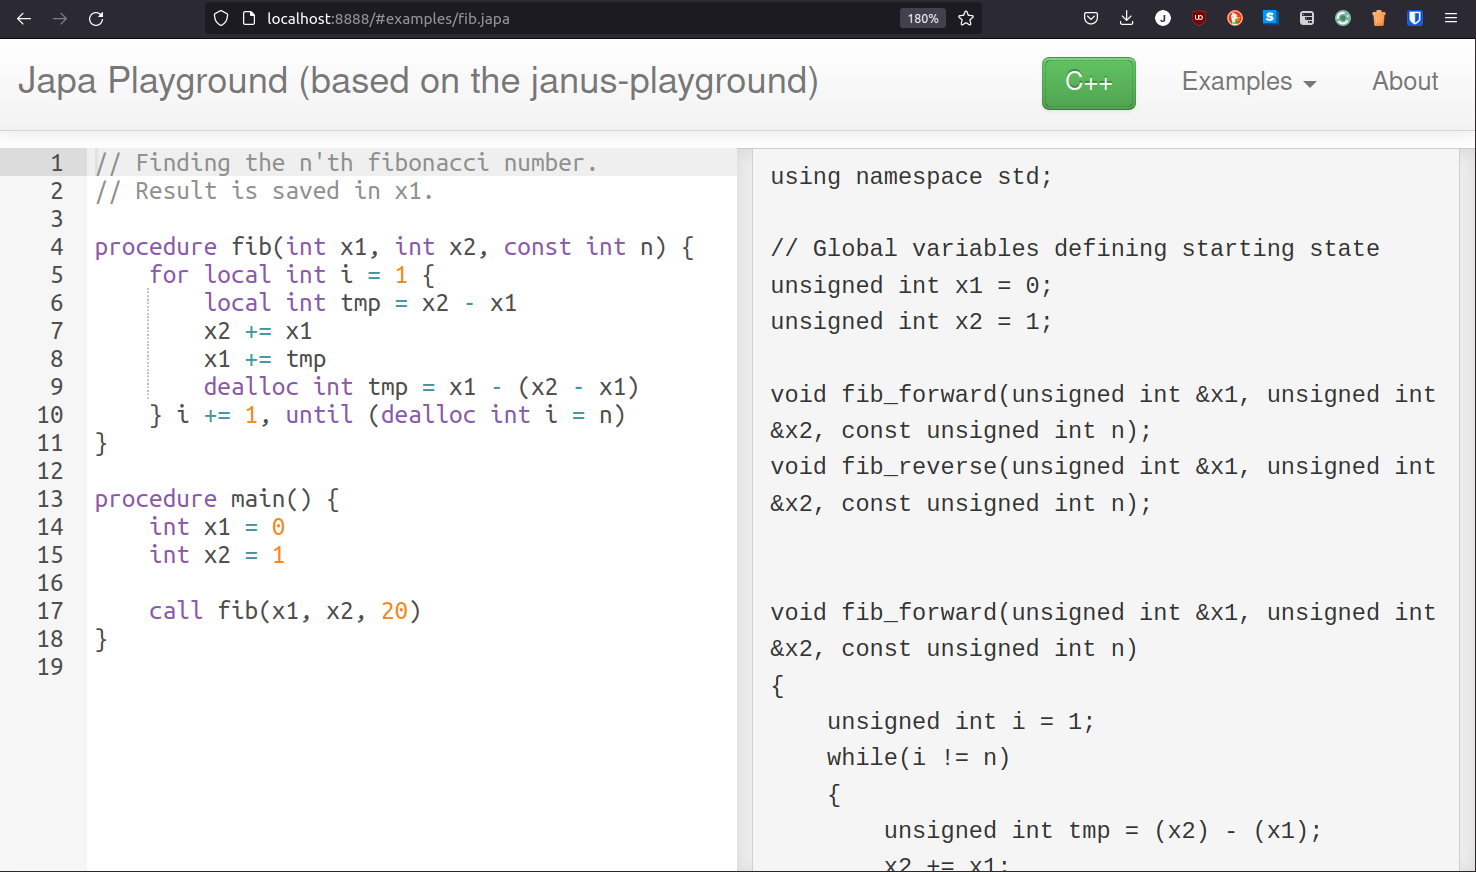
\includegraphics[width=\textwidth]{imgs/japa-playground.png}
    \caption{\lan playground allowing to write and translate \lan code to \texttt{C++}}
    \label{fig:japa-playground}
\end{figure}
\section{Reflection over project}
\section{Conclusion and future work }
This project presented the language \lan derived from the reversible language \texttt{Janus}.
\lan keeps the reversibility property derived from \texttt{Janus}, but changes e.g.\ the loop
construct in order to remove some runtime assertions directly from the language construct.

The \lan compiler presented in this project, translates from the source language into \texttt{C++}
code. It tries to remove runtime assertions by the use of the SMT solver \texttt{z3}. This is
done by recursing through the AST, translating into a \texttt{z3} model using its API for
\texttt{Haskell}. Each time a construct creating a runtime assertions is met, a query is made to
\texttt{z3}, in order to determine whether the assertion can be proven to always hold. This is
done by the steps:
\begin{enumerate}
      \item If it is a user-generated assertion, the assertion is checked to be satisfiable.
      \item The assertion is negated, and the \texttt{z3} model is checked to be satisfiable.
      \item If the negated assertion is not satisfiable, it means the assertion is always valid
            and can be optimized away.
\end{enumerate}
\noindent
In order to create a proper translation into \texttt{z3}, a simple type checker goes through the
AST before the optimization phase, both in order to (of cause) type check, but more importantly
annotate the AST with both types and array sizes.
\\
\\
Using the SMT solver \texttt{z3} the \lan compiler showed ability, to optimize most runtime
assertions away. The area in which the chosen method proved to be less effective, was when
analyzing reversed procedures. This probably stems from the fact, that the reversed procedure
some times work with "unspoken" starting contracts e.g.\ that the input numbers are always equal
when the forward procedure has been executed before.

Loop constructs also showed resistance towards optimizations, which makes sense, as \texttt{z3}
has no theory concerning loops. This means measures needed to be taken, in order to gather as much
information as safely possible, for \texttt{z3} to correctly validate assertions. In the best case
scenario loops were unrollable, so the pure information was retrievable, but in all other
cases, generalization methods was needed, to remove any possibly wrong information from the
SMT model.

This project showed great promise in regards to optimizing assertions away from imperative
reversible languages, but at present moment, the execution time of the compiler is rather slow.
For a simple Fibonacci program consisting of $21$ lines of code, the compile time was
$6.2$ seconds, with optimizations. This slow speed stem from the use of the \texttt{z3}
solver, and is probably caused by bad usage by the writer of this bachelor thesis.
\\
\\
The \lan language, as presented in this project, is rather simple, with simple types and
no recursion. For future work, implementing recursion would make sense, in crating a more
modern and pleasant language to work with. The slow execution time of the compiler should,
however, be a top priority, to improve development iteration time, to actually make the
optimization useful, as a "sparring" partner, to improve speed of developed code. As previously
mentioned the focus for this, should probably start at the use of \texttt{z3}, mainly of which
theories are called with the solver.

To avoid removing previously known information about variables, when analyzing loops that cannot
be unrolled, a method somewhat like the one presented in \cite{ai}, where loops are analyzed
using a combination of abstract interpretation and a SMT. This might be able to improve the
analysis of loops.


\subsection{Reflection over project }
After having completed this project, and experiencing the consequences of the workflow I
adopted, I can see that automated tests should probably have been implemented from the start.
The test section also reveals, the lack of unit tests for each function, as only the full
behavior of the compiler is tested. I fell in the trap, of ignoring setting up these tests
using \texttt{cabal}, as I simply felt swarmed already having to learn \texttt{Haskell}, \texttt{z3},
and all the other things needed for this thesis. I probably shouldn't have ignored it, as it lead
to some annoying bugs, when I finally implemented the tests of the full behavior.

As an extension to this, it would probably have been nice to work with more people on this
project, so I had someone to spar with on a daily basis.
\\
\\
Looking back it would probably have made sense to use \texttt{Boogie 2} instead of directly
communicating with \texttt{z3}. \texttt{Boogie 2} is a intermediate language representation, used
for verifying programming languages. Hence it works for multiple SMT solvers, and is used in
projects such as \texttt{Dafny}. Working with this intermediate language, might have made
it easier correctly modelling program structures. The reason why I did not chose it was, that
\lan is a reversible language, meaning it does not follow the ordinary program structure, meaning
representing the reversible semantics in the intermediate code might be unnecessary complicated.

\newpage
\bibliography{references}
\bibliographystyle{ieeetr}

\newpage
\section{Appendices} \label{sec:appendices}
% Test programs, test data, code, etc.
\subsection{Source Code}
\subsubsection{Main Function}
\lstinputlisting[language=Haskell]{../app/Main.hs}

\subsubsection{Syntax}
\lstinputlisting[language=Haskell]{../app/Syntax.hs}

\subsubsection{Parser}
\lstinputlisting[language=Haskell]{../app/Parser.hs}

\subsubsection{Type Checker}
\lstinputlisting[language=Haskell]{../app/TypeCheckAnnotate.hs}

\subsubsection{AST Reversing}
\lstinputlisting[language=Haskell]{../app/AstReversing.hs}

\subsubsection{Evaluating Constant Expressions}
\lstinputlisting[language=Haskell]{../app/EvalExpr.hs}

\subsubsection{Optimizer}
\lstinputlisting[language=Haskell]{../app/AssertionRemoval.hs}

\subsubsection{AST Renaming}
\lstinputlisting[language=Haskell]{../app/RenameProcedures.hs}

\subsubsection{\texttt{C++} Code Generation}
\lstinputlisting[language=Haskell]{../app/JapaToCpp.hs}

\subsubsection{Running tests}
\lstinputlisting[language=bash]{../bin/tester.sh}

\subsubsection{Makefile}
\lstinputlisting[language=bash]{../Makefile}

\subsubsection{Benchmark script}
\lstinputlisting[language=Bash, label={lst:runbenchmark}]{../benchmarks/runbenchmark.sh}


\end{document}

% Focus on the report now
% Interesting things are whatever goes beyond IPS course curriculum
% The uninteresting things needs to be mentioned, but no theory discussion for it!!

% In frontend only mention unconventional thing
% If the bug is hard to fix, don't spend half a week!!
%   then rather focus on the report!

% 4.3:
% Why on earth am I reversing the AST
% And how am I reversing (recursive descend)
%   How it happens precisely
% Setting it together with the overall approach of removing assertions.

% Maybe increase the font size or lessen the margins

% Use more code snippet in everything "new" e.g. loops
% TYPOS
% Typo in 4.4.1
% p.17
% Loop requirering -->
% Loop requiring
